\chapter{Instalacion y Configuracion}

En este Capitulo Aparte de guiarle para realizar una exitosa implementacion
Local del Servidor de Produccion se hara referencia a cada una de las
Herramientas y librerias Utilizadas.

\section{Requerimientos}

\subsection{Requerimientos de Hardware}

Cualquier equipo que cumpla con las Caracteristicas para correr Windows 7 es suficiente
en terminos de requerimientos minimos de Hardware siempre y cuando el numero de usarios
esperados no sea alto, despues el resto dependera de sus necesidades.\\[0.5cm]

\begin{itemize}
    \item Procesador x86, x64 de 1 Ghz o superior.
    \item Memoria Ram 1 GB o Superior 
\end{itemize}


\subsection{Requerimientos de Software}


\begin{itemize}
    \item Apache 2.2
    \item PosgreSQL 9.2
    \item Python 2.7.x o Python 2.6.x
    \item Django 1.3.x o Superior
    \item PGAdmin
    \item psycopg2
    \item mod\_wsgi
    \item ReportLab
    \item easy\_thumbnails
    \item django\_extensions
    \item django\_cron
\end{itemize}


\section{Apache}

Existen 2 caminos para instalar Apache La Primera Hacer una instalacion Limpia
de Apache, la 2da es cuando no se quiere trastear con tanta configuracion por lo que
opta por infraestructuras tipo WAMP, LAMP, WAPP, etc.

\subsection{Instalacion en Limpio}

Solo recomiendo este tipo de instalacion desde 0 para quienes ya poseen un conocimiento
avanzado en cuanto a manejo de servidores.

Descargamos de \url{Apache.org} la ultima version disponible, puedes utilizar el siguiente
vinculo: \url{http://www.apachehaus.com/cgi-bin/download.plx}. \\ 

Crea dos carpetas en la unidad C, la primera de nombre {\bfseries Apache} y la segunda
{\bfseries servidor}. Descomprime el archivo descargado y ejec\'utalo,
sigue los pasos de la instalaci\'on y de los datos que te piden solo escoge el
destino de la instalaci\'on, que ser\'a la carpeta que creaste en
{\bfseries C:\textbackslash Apache }, los otros datos d\'ejalos de la forma
predeterminada para configurarlos m\'as tarde.
El programa al instalarse crea un icono en el área de notificación que te
permitir\'a: iniciar, detener y reiniciar Apache; tienes que tener en cuenta que
cualquier cambio que hagas en el archivo de configuración no tendrá efecto
hasta que reinicies el servidor.

\subsection{Instalacion mediante WAMP, LAMP, MAMP, WAPP}

Existem una infinidad de Paquetes precompilados y configurados, con Apache, PHP, PosgreSQL o MySQL y mas.
Dichas infraestructuras suelen nombrarse como el acronomico de las herramientas que agrupan por ejemplo:\\[1cm]

\begin{itemize}
    \item {\large WAMP {\bfseries W}indows {\bfseries A}pache {\bfseries M}ySQL {\bfseries P}HP}
    \item {\large WAPP  {\bfseries W}indows {\bfseries A}pache {\bfseries P}osgreSQL {\bfseries P}HP}  
    \item {\large LAMP {\bfseries L}inux {\bfseries A}pache {\bfseries M}ySQL {\bfseries P}HP} 
    \item {\large MAMP {\bfseries M}ac OS {\bfseries A}pache {\bfseries M}ySQL {\bfseries P}HP}  
\end{itemize}


Algunas distribuciones mas usadas disponibles Para Windows son WAMP Server \url{http://www.wampserver.com/} (WAMP),
XAMPP \url{http://sourceforge.net/projects/xampp/} (WAMP + Perl), Bitnami \url{http://bitnami.com/stack/wapp} (WAPP)
solo nos resta elegir cualquiera de ellas e instalarlas, aparte de la ruta de instalacion nos pediran el usuario y
contraseña para acceder al motor de Base de Datos.

\subsection{Configuracion}

Toda la configuración para el funcionamiento de Apache se guarda en un archivo
de texto nombrado: {\bfseries httpd.conf} que se encuentra en la ruta
{\bfseries C:\textbackslash Apache \textbackslash conf } si realizamos una instalacion en limpio o
{\bfseries C:\textbackslash wamp \textbackslash bin \textbackslash  Apache \textbackslash conf } si
instalamos el paquete multiple preconfigurado no es necesario realizar este paso por lo
que lo podremos salta.\\

Al archivo {\bfseries httpd.conf} lo podemos editar en cualquier editor de texto como Notepad.

Buscamos la linea que dice

\begin{lstlisting}[style=consola, numbers=none]
    Listem LocalHost:80
\end{lstlisting}

y la Cambiamos por:

\begin{lstlisting}[style=consola, numbers=none]
    Listem 80
\end{lstlisting}

Ahora buscamos la instruccion:

\begin{lstlisting}[style=consola, numbers=none]
    DocumentRoot "C:\xxxxxxxx"
\end{lstlisting}

y la Cambiamos por:

\begin{lstlisting}[style=consola, numbers=none]
    DocumentRoot "C:\Servidor"
\end{lstlisting}

Recordar que al inicio de la instalacion creamos una Carpeta llamada Servidor en
la unidad C. Por ultimo solo nos queda reiniciar el servidor Apache e introducir
la siguiente direccion \url{http://127.0.0.1} si nos aparece una pagina
{\bfseries It's Work!} felicidades Apache esta Funcionando.


\subsection{Instalacion de PosgreSQL}

La versión de PostgreSQL que he utilizado durante el desarrollo del sistema es
la 9.2.x, quisas cuando leas esto haya salido una nueva version la cual no deberia
generar inconvenientes ademas de que es posible que el proceso de instalación
pueda variar.\\[0.2cm]
 
El primer paso es descargar el instalador de PostgreSQL para Windows,
lo puedes descargar desde el enlace siguiente
\url{http://www.postgresql.org/download/windows}, nos bajara un instalador similar
a {\bfseries postgresql-9.2.3-rc1-windows.exe} lo ejecutamos como administrador.\\[0.2cm]

Si tenemos activado el control de cuentas de usuario nos mostrar\'a una advertencia
con el texto "¿Desea permitir que este programa realice cambios en el equipo?",
pulsaremos "Sí" para continuar con la instalación de PostgreSQL.\\[0.2cm]

Indicaremos la carpeta de instalaci\'on de PostgreSQL, donde se guardarán los
ejecutables, librer\'{\i}as y ficheros de configuraci\'on de PostgreSQL en mi caso el
directorio es {\bfseries C: \textbackslash PosgreSQL \textbackslash 9.2 },
Indicaremos tambi\'en la carpeta donde se guardarán los datos por defecto
de PostgreSQL {\bfseries C: \textbackslash psql-data }.\\[0.2cm]

Solo nos queda introducir la contraseña para el superusuario "postgres" que
será con el que iniciemos sesión para administrar la base de datos, despues
podremos crear otros usuarios si es necesario. Ademas introduciremos el puerto
de escucha para la conexión con el servidor PostgreSQL, por defecto el 5432.\\[0.2cm]

Seleccionaremos la configuración regional y comenzara la instalacion, con esto
PosgreSQL quedara instalado. Si tenemos algún cortafuegos (firewall) deberemos
abrir el puerto 5432.

\subsection{Creacion de la Base de Datos}

Junto con la Instalacion de PosgreSQL se instala el PGAdmin III que es una Heramienta
GUI para administrar el motor de base de Datos. Iniciamos el Programa,
desplegaremos "Server Groups", dentro desplegaremos "Servidores" y dentro de
éste pulsaremos con el botón derecho del ratón sobre "PostgreSQL 9.0 (localhost:5432),
en el menú emergente seleccionaremos "Conectar".

Introduciremos la contraseña para el superusuario postgres
(la contraseña introducida en la instalación).

Pulsaremos con el botón derecho del ratón sobre "Bases de datos", seleccionaremos
"Nueva Base de Datos", en la pestaña "Propiedades" introduciremos los
siguientes datos:

\begin{itemize}
    \item Nombre: nombre de la base de datos, en nuestro caso "BDSem".
    \item Propietario: seleccionaremos el usuario creado anteriormente "posgres".
    \item Codificado: seleccionaremos UTF8.
    \item Tablespace: seleccionaremos el tablespace creado anteriormente "pg\_default".
    \item Colación: seleccionaremos "Spanish, Argentina".
    \item Tipo carácter: seleccionaremos "Spanish, Argentina".
\end{itemize}

Pulsaremos OK para crear la base de datos, con esto ya tendremos nuestra base
de datos aunque vacia, el resto como creacion de las Tablas correspondientes
nesesarias para el proyecto lo haremos mas adelante mediante Django.



\section{Instalacion de Python}

Para este proyecto se utilizo CPython pero no la version Oficial url{http://www.python.org}
sino la que distribuye Active State \url{http://www.activestate.com} llamada
{\bfseries Active Python} la cual provee caracteristicas adicionales a version oficial,
podremos descargar la ultima version desde \url{http://www.activestate.com/activepython/downloads}
aunque se recomienda instalar la version 2.7.x para evitar cualquier posible problema.

\subsection{Probando Python}
Para probar que la instalacion haya sido correcta abriremos la Terminal "cmd.exe"
y escribiremos:

\begin{lstlisting}[style=consola, numbers=none]
    python
\end{lstlisting} 

Si todo va bien nos debera aparecer algo similar a:

\begin{figure}[h]
    \centering
    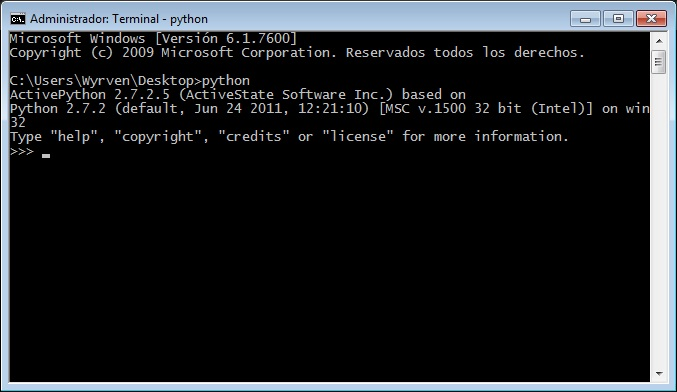
\includegraphics[scale=0.7]{resourse/consola-python.jpg}
    \caption{Ejecutando Python en la Terminal}
    \label{fig:01}
\end{figure}    

En caso contrario deberias revisar que la ruta de Python este dentro de la variable
 PATH del sistema.




